\documentclass[border=3pt]{standalone}
% Shared style for all figures: Latin Modern to match the manuscript, and the
% Okabe-Ito colour-blind-safe palette.
\usepackage{lmodern}
\usepackage[T1]{fontenc}
\usepackage{pgfplots}
\usepackage{pgfplotstable}
\pgfplotsset{compat=1.18}
\usetikzlibrary{positioning,arrows.meta,fit,calc,backgrounds,patterns}
\definecolor{oiblue}{HTML}{0072B2}
\definecolor{oiorange}{HTML}{E69F00}
\definecolor{oigreen}{HTML}{009E73}
\definecolor{oivermillion}{HTML}{D55E00}
\definecolor{oisky}{HTML}{56B4E9}
\definecolor{oipurple}{HTML}{CC79A7}
\definecolor{oigrey}{HTML}{999999}
\pgfplotsset{every axis/.append style={font=\small, tick label style={font=\footnotesize},
  label style={font=\small}, legend style={font=\footnotesize, draw=none}}}

\hyphenpenalty=10000
\exhyphenpenalty=10000
\begin{document}
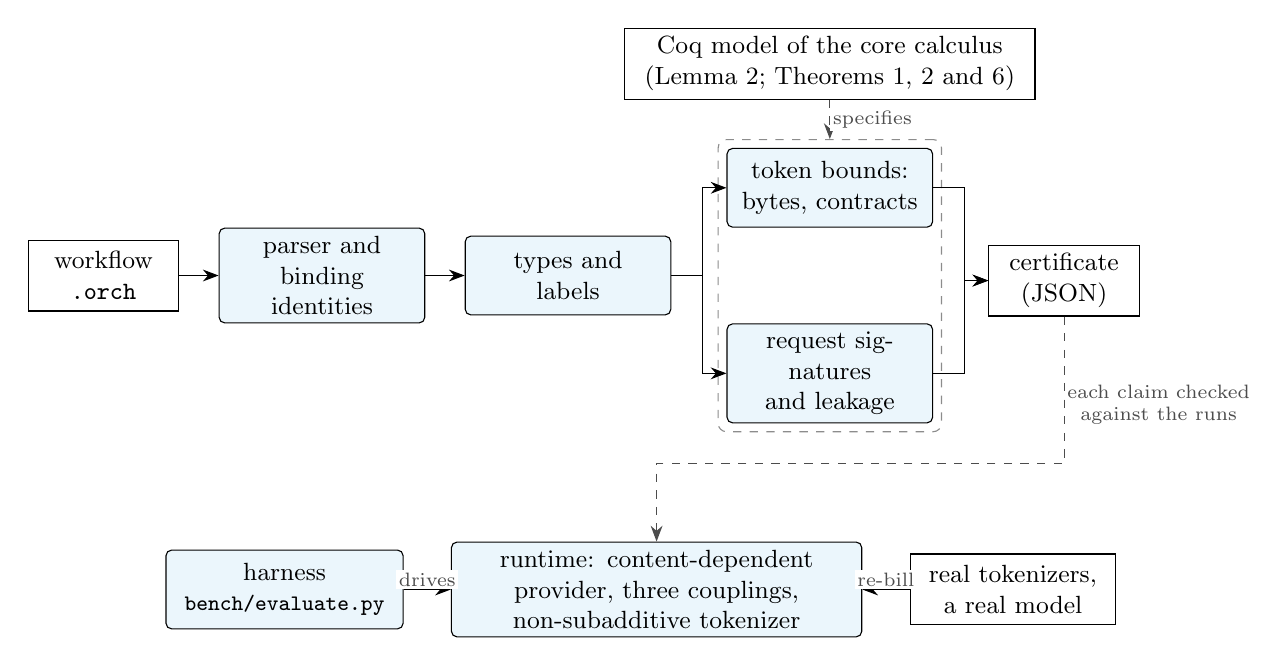
\begin{tikzpicture}[
    font=\small, >={Stealth[length=2mm]},
    every node/.style={align=center},
    stage/.style={draw, rounded corners=2pt, fill=oisky!12, minimum height=10mm,
                  inner sep=3pt, text width=24mm},
    art/.style={draw, fill=white, minimum height=9mm, inner sep=3pt, text width=17mm},
    check/.style={->, dashed, black!70},
    lab/.style={font=\scriptsize, text=black!70, fill=white, inner sep=1pt}]
  \node[art] (src) {workflow\\\texttt{.orch}};
  \node[stage, right=5mm of src] (parse) {parser and\\binding identities};
  \node[stage, right=5mm of parse] (labels) {types and\\labels};
  \node[stage, above right=1mm and 7mm of labels] (cost) {token bounds:\\bytes, contracts};
  \node[stage, below right=1mm and 7mm of labels] (rel) {request signatures\\and leakage};
  \node[art, right=7mm of $(cost.east)!0.5!(rel.east)$] (cert) {certificate\\(JSON)};
  \draw[->] (src) -- (parse);
  \draw[->] (parse) -- (labels);
  \draw[->] (labels.east) -- ++(4mm,0) |- (cost.west);
  \draw[->] (labels.east) -- ++(4mm,0) |- (rel.west);
  \draw[->] (cost.east) -- ++(4mm,0) |- (cert.west);
  \draw[->] (rel.east) -- ++(4mm,0) |- (cert.west);
  % the two analyses, grouped; the Coq model specifies both
  \begin{scope}[on background layer]
    \node[draw, dashed, rounded corners=3pt, black!45, inner sep=3pt, fit=(cost)(rel)] (analyses) {};
  \end{scope}
  \node[art, text width=50mm, above=5mm of analyses] (coq) {Coq model of the core calculus\\(Lemma 2; Theorems 1, 2 and 6)};
  % runtime and harness
  \node[stage, text width=50mm, below=15mm of rel, xshift=-22mm] (run) {runtime: content-dependent\\provider, three couplings,\\non-subadditive tokenizer};
  \node[stage, text width=28mm, left=6mm of run] (harness) {harness\\\texttt{\footnotesize bench/evaluate.py}};
  \node[art, text width=24mm, right=6mm of run] (real) {real tokenizers,\\a real model};
  \draw[->] (harness) -- node[lab, above]{drives} (run);
  \draw[->] (real) -- node[lab, above]{re-bill} (run);
  \coordinate (turn) at ([yshift=-4mm]analyses.south -| run.north);
  \draw[check] (cert.south) |- node[lab, right, pos=0.3]{each claim checked\\against the runs} (turn) -- (run.north);
  \draw[check] (coq.south) -- node[lab, right]{specifies} (analyses.north);
\end{tikzpicture}
\end{document}
